% Compile with XeLaTeX (fontspec + TeX--XeT for right-to-left snippets):
%   xelatex main && bibtex main && xelatex main && xelatex main
\documentclass[11pt]{article}
\usepackage[preprint]{acl}

% ---------- fonts (Times-compatible main font; Hebrew/Arabic with full mark support)
\usepackage{fontspec}
\setmainfont{TeX Gyre Termes}
\newfontfamily\hebfont[Path=fonts/, Script=Hebrew, BoldFont=DavidLibre-Bold.ttf]{DavidLibre-Regular.ttf}
\newfontfamily\arabfont[Path=fonts/, Script=Arabic, Scale=0.97, BoldFont=Amiri-Bold.ttf]{Amiri-Regular.ttf}
\TeXXeTstate=1
\newcommand{\he}[1]{\mbox{\beginR\hebfont #1\endR}}
\newcommand{\ar}[1]{\mbox{\beginR\arabfont #1\endR}}

\usepackage{microtype}
\usepackage{placeins}
\usepackage{graphicx}
\usepackage{booktabs}
\usepackage{amsmath}
\usepackage{multirow}
\usepackage{makecell}
\newcommand{\est}[3]{\makecell[c]{$#1$\\[-2pt]{\scriptsize[$#2$, $#3$]}}}
\usepackage{xcolor}
\usepackage{pifont}
\usepackage{tikz}
\usetikzlibrary{positioning,arrows.meta,calc}
\definecolor{heblue}{HTML}{2A78D6}
\definecolor{arorange}{HTML}{EB6834}
\definecolor{ink2}{HTML}{52514E}
\definecolor{panel}{HTML}{F4F3F0}
\definecolor{good}{HTML}{0CA30C}
\definecolor{bad}{HTML}{D03B3B}
\newcommand{\cmark}{\textcolor{good}{\ding{51}}}
\newcommand{\xmark}{\textcolor{bad}{\ding{55}}}
\newcommand{\U}{\textsc{u}}
\newcommand{\D}{\textsc{d}}
\newcommand{\cA}{\textsf{A}}
\newcommand{\cB}{\textsf{B}}
\newcommand{\cC}{\textsf{C}}
\newcommand{\cD}{\textsf{D}}
\newcommand{\ci}[2]{\mbox{[$#1$, $#2$]}}

\title{Lost in Vocalization: Optional Diacritics Disrupt\\Hebrew and Arabic Factual Recall in Aya-23-8B}

\author{Anonymous research team}

\begin{document}
\maketitle

\begin{abstract}
Hebrew and Arabic are usually written without their optional diacritics, the
small marks that spell out vowels and pronunciation. Adding these marks to an
entity's name keeps the entity, the fact and the language fixed but roughly
triples the number of subword tokens in the name: a controlled test of whether
factual recall depends on how the subject is written. We test
Aya-23-8B on five sets of facts with no shared subjects: 123 reviewed place facts
(a pilot, a held-out test and a Google-RE set) and two sets checked against
independent sources, 184 Arabic city--country and 240 Hebrew
locality--subdistrict facts. Marking lowers the log-likelihood of the correct
answer by 1.35 to 1.64 nats on the pilot and held-out subjects, and its margin
over a fixed wrong answer by 1.37 nats on the Arabic cities (Holm $p=.001$),
where exact accuracy falls from 26.6\% to 16.3\% (descriptive). On the Hebrew localities, where baseline accuracy is very low (3.3\%), the effects are uncertain.
Restoring the unmarked state at the subject's last token in layers 12--13,
a window chosen on the pilot, recovers about 1.3 nats on held-out and new Arabic
subjects. Two exploratory decompositions show that the loss is sensitive to how
the letters are split into tokens. Splitting the unmarked name at the token
boundaries the marks induce gives an estimated loss close to marking's, while the average of an early and a late artificial split of the unmarked
name, each with the marked name's token count, scores 1.0 to 2.3 nats below the
marked name. These splits also change which tokens
appear, so they cannot separate count from identity.
\end{abstract}

\section{Introduction}
\label{sec:intro}

Multilingual language models often know a fact in English but give a wrong
answer when asked in another language
\citep{jiang-etal-2020-x,kassner-etal-2021-multilingual,qi-etal-2023-cross}.
Mechanistic studies explain part of this gap: much of the processing happens in a
largely shared representation, which is converted into the target language only
in late layers
\citep{wendler-etal-2024-llamas,dumas-etal-2025-separating,wang-etal-2025-lost-multilinguality}.
For factual recall, \citet{fierro-etal-2025-multilingual} report that
\emph{subject enrichment}, the early-layer process that gathers attributes of the
subject into its last token \citep{geva-etal-2023-dissecting}, does not depend on
the language. These conclusions, however, come from facts the models already
recall and from the standard written form of each subject.

Hebrew and Arabic offer a clean test of whether the written form matters. Both
are written in \emph{abjads}, scripts whose letters record consonants and leave
many vowels unwritten. Vowels, doubled consonants and some pronunciation details
can be added with optional diacritics, small marks above, below or inside
the letters (Hebrew \emph{niqqud}, Arabic \emph{tashkil}). Everyday text omits
them, while teaching materials, religious texts and poetry often include them
\citep{habash-2010-introduction,gershuni-pinter-2022-restoring}. We compare an
unmarked (\U) and a marked (\D) spelling of the same entity's name. The entity,
the fact, the language, the script and the entity's popularity stay the same,
while the tokenizer splits the name differently: with the Aya-23 tokenizer,
marking raised the number of subject tokens in all 1{,}586 prompt pairs we built
(Figure~\ref{fig:overview}). Comparing two spellings of one entity avoids the
frequency confound of comparisons between entities
\citep{kandpal-etal-2023-longtail,mallen-etal-2023-trust}, although it also
changes how familiar the spelling is.

\begin{figure*}[t]
\centering
\begin{minipage}[b]{0.605\textwidth}
\centering
\begin{tikzpicture}[font=\footnotesize, >=Stealth,
  box/.style={draw=ink2!60, rounded corners=2pt, fill=white, inner sep=3pt, align=center},
  model/.style={draw=ink2, rounded corners=2pt, fill=panel, minimum width=1.35cm, minimum height=0.95cm, align=center, inner sep=2pt},
  lab/.style={font=\scriptsize, text=ink2}]
\node[box, text width=3.05cm] (pu) {\textbf{\U}\enspace \he{אוניברסיטת מקגיל}\\[-1pt]{\scriptsize\textcolor{ink2}{4 subject tokens}}};
\node[model, right=0.42cm of pu] (mu) {Aya-23-8B\\[-1pt]{\scriptsize 32 layers}};
\node[box, right=0.42cm of mu, text width=2.2cm] (au) {\he{מונטריאול}\\[-1pt]{\scriptsize Montreal \cmark}};
\node[box, below=0.95cm of pu, text width=3.05cm] (pd) {\textbf{\D}\enspace \he{אוּנִיבֶרְסִיטַת מֶקְגִיל}\\[-1pt]{\scriptsize\textcolor{ink2}{20 subject tokens}}};
\node[model, right=0.42cm of pd] (md) {Aya-23-8B\\[-1pt]{\scriptsize 32 layers}};
\node[box, right=0.42cm of md, text width=2.2cm] (ad) {\he{אירלנד}\\[-1pt]{\scriptsize Ireland \xmark}};
\draw[->, thick, ink2] (pu) -- (mu); \draw[->, thick, ink2] (mu) -- (au);
\draw[->, thick, ink2] (pd) -- (md); \draw[->, thick, ink2] (md) -- (ad);
\draw[->, very thick, heblue, dashed] ($(mu.south)+(-0.2,0)$) -- node[right, font=\scriptsize, text=heblue, align=left, xshift=1pt]{E5: copy the state at the subject's\\last token, layers $\ell,\ell{+}1$} ($(md.north)+(-0.2,0)$);
\node[lab, above=0pt of pu] {McGill University (Q201492), HQ question};
\node[lab, above=0pt of au] {greedy answer};
\node[lab, below=1pt of pd, align=center] {same base letters, niqqud added};
\node[lab, below=1pt of ad, align=center] {$\log P(\text{Montreal})$: $-0.13 \rightarrow -9.16$};
\end{tikzpicture}
\end{minipage}\hfill
\begin{minipage}[b]{0.375\textwidth}
\centering
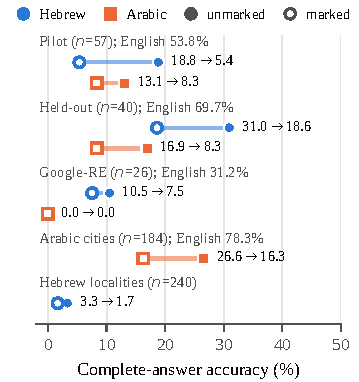
\includegraphics[width=\linewidth]{figures/fig1_accuracy.pdf}
\end{minipage}
\caption{\textbf{Left:} the paired design. The same question is asked with an
unmarked (\U) or a marked (\D) subject name; in this pilot example (Hebrew),
marking raises the subject from 4 to 20 tokens and turns a correct answer into a
wrong one. \textbf{Right:} accuracy with unmarked (filled) and marked (open)
names, with English for reference;
relation-macro over three prompts (reviewed cohorts) or template~1
(source-checked cohorts).}
\label{fig:overview}
\end{figure*}

We ask three questions. \textbf{RQ1:} Does marking a subject's name change
Aya-23-8B's ability to recall a fact about it? \textbf{RQ2:} Is the change
explained by the number of subword tokens? \textbf{RQ3:} Is the deficit carried
by the hidden state at the subject's last token? We investigated these questions in an exploratory pilot of 57 facts,
then evaluated the findings on 40 held-out subjects frozen before Aya was run on
them, on a second benchmark archive and on 424 facts from independent
sources. We contribute (i) 547 place facts with paired unmarked and
marked names (\S\ref{sec:data}); (ii) a paired evaluation of answers,
likelihoods and margins, with controlled activation patching and an exact
decomposition of the marking effect (\S\ref{sec:methods}); and (iii) results
showing that marking lowers the evidence for the correct answer on independent
subjects and that restoring the unmarked state at the subject's last token, at a
window chosen in advance, recovers much of the loss, with exploratory evidence that the loss is
sensitive to how the letters are split
(\S\ref{sec:results}).\footnote{Code, data, protocols and Aya result archives,
with instructions for reproducing the results:
\url{https://github.com/mais-asli/fragmented-facts-aya-public}.}

\section{Background and Related Work}
\label{sec:related}

\paragraph{Factual recall in language models.}
Fill-in-the-blank (cloze) probing showed that pretrained models store relational facts
\citep{petroni-etal-2019-language}, and multilingual versions of these probes
found much lower and less consistent recall outside English
\citep{jiang-etal-2020-x,kassner-etal-2021-multilingual,qi-etal-2023-cross}.
Feed-forward (MLP) layers act as key--value memories \citep{geva-etal-2021-transformer}, causal
tracing points to middle-layer MLPs at the last subject token
\citep{meng-etal-2022-locating}, and attention knockout separates three stages:
subject enrichment, relation propagation and attribute extraction
\citep{geva-etal-2023-dissecting}. Directions in the hidden states that signal
whether an entity is known also predict whether a model answers or abstains
\citep{ferrando-etal-2025-know}. Such interventions \citep{vig-etal-2020-causal}
depend on the corruption, metric and controls
\citep{zhang-nanda-2024-best,heimersheim-nanda-2024-patching}.

\paragraph{Multilingual recall.}
Llama-2 appears to process non-English prompts through an English-biased concept
space \citep{wendler-etal-2024-llamas}, patching can separate a concept from its
output language \citep{dumas-etal-2025-separating}, and many cross-lingual
inconsistencies arise late, when the answer is converted into the target
language \citep{wang-etal-2025-lost-multilinguality}.
\citet{fierro-etal-2025-multilingual} find subject enrichment to be
language-independent, but they studied only facts the models predicted correctly
and excluded Hebrew for both decoder-only models because too few facts were
recalled. The claim has not been tested under a change of written form.

\paragraph{Tokenization and detokenization.}
Subword tokenizers \citep{sennrich-etal-2016-neural} give some languages much
more of their vocabulary than others, and heavier fragmentation (more tokens per
word) is linked to worse performance and higher cost
\citep{rust-etal-2021-good,ahia-etal-2023-languages,petrov-etal-2023-unfairness}.
Models rebuild multi-token words internally: \citet{kaplan-etal-2025-tokens} find
a \emph{detokenization} stage that forms each word's representation at its last
token in early and middle layers, and \citet{feucht-etal-2024-token} show that
token-level information about multi-token words and entities is erased early.
Instruction-tuned models also keep most of their performance under non-standard splits, even into single characters
\citep{zheng-etal-2025-broken}.

\paragraph{Diacritics in Hebrew and Arabic NLP.}
Both languages are morphologically rich, with many prefixes and suffixes attached
to words, and are usually written without vowel marks
\citep{habash-2010-introduction,tsarfaty-etal-2020-spmrl,seker-etal-2022-alephbert}.
Restoring the marks (diacritization) is a standard task
\citep{gershuni-pinter-2022-restoring}, and \citet{bondok-etal-2025-proper}
release gold diacritized forms of Arabic Wikipedia proper names.
\citet{gorman-pinter-2025-dont} argue that inconsistent Unicode encoding of the
marks, and their blanket removal during preprocessing, harm multilingual models.
Closest to our work, \citet{inoue-etal-2026-diacritics} show for Arabic that
full automatic diacritization increases fragmentation, lowers representational
similarity and hurts most of nine LLMs on multiple-choice benchmarks, and
\citet{alakeel-etal-2026-morphemes} caution that aligning Arabic tokens with
morphemes, the smallest units that carry meaning or grammatical information, is
neither necessary nor sufficient for generating correct word forms.
We mark only the subject's name, measure open-ended recall, add Hebrew, and use
causal controls and independent test sets.

\section{Data}
\label{sec:data}

All facts ask for a place and have a single answer that independent sources support, at the level of detail they give. Table~\ref{tab:data}
summarizes the five cohorts; no subject appears in more than one.

\paragraph{Reviewed cohorts.}
The first three cohorts use four Wikidata relations
\citep{vrandecic-krotzsch-2014-wikidata}: place of birth (P19), place of death
(P20), headquarters location (P159) and location of formation (P740), with
answers that held before Aya's release in May 2024. The \textbf{pilot} (57
facts) comes from 70 mLAMA facts available in English, Hebrew and Arabic
\citep{kassner-etal-2021-multilingual}. The \textbf{held-out test} keeps 40 of 60
further mLAMA candidates from a test split fixed in advance; its facts,
spellings, prompts, scorer and analysis plan were frozen before Aya was run on
those candidates. The \textbf{Google-RE} cohort (26 of 32 candidates) draws birth and death
facts, in a fixed pseudo-random order, from a second archive distributed with
LAMA \citep{petroni-etal-2019-language}. For each subject and language, \D{} fully marks \U{} with vowel and
pronunciation marks from a fixed list, without adding, removing or changing any
letter (Appendix~\ref{app:cohorts} explains each mark). Every fact, answer name and
spelling pair was checked against a cited source before its freeze.

\paragraph{Source-checked cohorts.}
Two further cohorts take both the fact and the marked name from independent
sources. An item was kept only if the sources agreed and it passed fixed spelling
rules, and every kept item was then verified against those sources
(Appendix~\ref{app:cohorts}). \textbf{Arabic cities} (184 facts, 72 countries)
link the gold diacritized proper names of CP-WIKI-D3K
\citep{bondok-etal-2025-proper} to Wikidata and GeoNames \citep{geonames-2026};
country names and accepted variants come from Unicode CLDR \citep{cldr-2026}.
\textbf{Hebrew localities} (240 facts, 14 subdistricts) link the 2023 locality
file of the Israeli Central Bureau of Statistics \citep{cbs-2023-localities},
which gives each locality's official subdistrict, to the marked name in the
opening sentence of the locality's Hebrew Wikipedia article. Each fact also has
a \emph{distractor}, one fixed wrong answer chosen before any output for its
cohort: a neighboring or same-continent country, or another subdistrict.

\begin{table*}[t]
\centering\footnotesize
\setlength{\tabcolsep}{4.4pt}
\renewcommand{\arraystretch}{1.02}
\begin{tabular}{@{}lccccc@{}}
\toprule
 & Pilot & Held-out & Google-RE & Arabic cities & Hebrew localities\\
\midrule
Sources & mLAMA & mLAMA & Google-RE & CP-WIKI-D3K, GeoNames & CBS, Wikipedia\\
Facts (per relation) & 57 (14/15/14/14) & 40 (11/13/6/10) & 26 (14/12/--/--) & 184 & 240\\
Languages; templates & he, ar; 3 & he, ar; 3 & he, ar; 3 & ar; 2 & he; 2\\
Distinct answers & 47 & 28 & 13 & 72 & 14\\
Tokens \U$\to$\D, he & 5.9$\to$18.5 & 6.3$\to$20.8 & 5.5$\to$17.3 & -- & 3.2$\to$10.2\\
Tokens \U$\to$\D, ar & 5.5$\to$17.5 & 5.6$\to$17.4 & 5.6$\to$15.6 & 3.5$\to$9.2 & --\\
Prompt pairs & 342 & 240 & 156 & 368 & 480\\
English recall & 17 (31) & 16 (21) & 6 (8) & 144 & --\\
Median 2023 views & 80k & 64k & 7k & -- & --\\
\bottomrule
\end{tabular}
\caption{The five cohorts. Relations: P19/P20/P159/P740 (reviewed cohorts),
city--country and locality--subdistrict. Tokens: mean Aya tokens overlapping the
subject in the full prompt. English recall: facts answered by both (at least one) of two English screening
prompts, or by one English control prompt (Arabic cities). Views: English
Wikipedia.}
\label{tab:data}
\end{table*}

\paragraph{Prompts.}
The reviewed cohorts use three templates per relation and language (``Subject:
\{subject\} / Question: \dots / Give only the place name.''). The subject comes
before the question, so the subject's last token cannot attend to the relation. Eight separate English screening prompts define an
\emph{English-recallable} core of facts for
sensitivity analyses. The source-checked cohorts use two native questions each,
such as ``In which country is \{subject\} located?'', with one English control prompt for the Arabic cities
(Appendix~\ref{app:templates}).

\section{Methods}
\label{sec:methods}

\paragraph{Model and inference.}
We study Aya-23-8B \citep{aryabumi-etal-2024-aya23}, an open-weight decoder-only
model instruction-tuned for 23 languages, including Hebrew and Arabic
(checkpoint \texttt{CohereLabs/aya-23-8B}, revision \texttt{89da1a0}; 32 layers;
a 256k-token byte-level BPE vocabulary; rotary position embeddings). We use the official chat template, greedy decoding (at most 24 tokens), and 4-bit NF4 weights with FP16 computation
\citep{dettmers-etal-2023-qlora} on one 11\,GB GPU.

\paragraph{Outcomes.}
\emph{Complete-answer accuracy} requires the whole generated answer, after
conservative normalization, to exactly match an accepted name of the gold
entity. The
\emph{answer log-likelihood} of a fixed answer $a$ given a prompt $x$ is
$S(a\mid x)=\sum_{j}\log P(a_j\mid x,a_{<j})$, computed by feeding the answer
tokens after the prompt. The same answer tokens are scored for \U{} and \D{}, so
$\Delta S=S(a\mid x_\D)-S(a\mid x_\U)$ reflects only the change in the input.
Values are in nats (natural-log units); a change of $-1.4$ nats makes the answer
about four times less likely. For the source-checked cohorts the primary outcome
is the \emph{margin} of the gold answer $a$ over the distractor $b$,
$M(x)=S(a\mid x)-S(b\mid x)$, and its change $\Delta M=M(x_\D)-M(x_\U)$, which
measures the evidence for the correct answer relative to one alternative chosen
in advance.

\paragraph{Experiments.}
\textbf{E1} evaluates unmarked prompts in the target language and, where
available, in English. \textbf{E2} evaluates the \U/\D{} pairs in every cohort. \textbf{E3} splits one token of an unmarked prompt into
two tokens with the same bytes, inside or outside the subject
(Appendix~\ref{app:e3}). \textbf{E4} replaces the subject of an English prompt by
another subject and restores the original state at one position and layer: the
subject's first or last token, or the \emph{prediction position} (the prompt
position used to predict the first answer token).
\textbf{E5} is activation patching: it copies the residual stream, the hidden
state that each layer reads and updates, from the \U{} run at the subject's last
token into the \D{} run at two consecutive layers (4--5, 12--13, 20--21 or
28--29, counted from zero). Its controls are an identity sham (\D$\to$\D), an unrelated donor (a subject with a different answer), the same patch at the first subject token or at the delimiter after the subject, and the reverse
patch (\D$\to$\U); the source-checked runs use the sham, unrelated-donor and
first-token controls. Each condition is compared with its unpatched run, as a harmful donor can inflate a same-minus-unrelated gap.

\textbf{E6} splits the marking effect into three exact steps. In every marked
name the tokenizer places the marks in separate tokens that contain only marks,
so deleting these tokens leaves a sequence that decodes exactly to the unmarked
name (all 246 fact--language pairs of the reviewed cohorts). We compare four
inputs. \cA{} is the unmarked prompt, split as the tokenizer normally splits it.
\cB{} is the same unmarked text, split into the letter tokens of \D{} (\D{}
with its mark tokens removed). \cC{} keeps the tokens of \cB{} at the positions
they occupy in \D{}, leaving gaps where the marks were. \cD{} is the marked
prompt. Each step changes one thing: \cA$\to$\cB{} how the fixed text is split,
\cB$\to$\cC{} the positions of fixed tokens, and \cC$\to$\cD{} the presence of
the mark tokens (\cC{} behaves as \D{} with all attention to the marks blocked). The three steps add up to the template-1 E2 effect. \textbf{E7} adds three splits of the same unmarked text:
\textsf{mid}, halfway between the token counts of \cB{} and \D, and two \textsf{full} splits with exactly \D's subject and prompt token counts,
placing the extra boundaries early or late in the name. Since \D{} has more
tokens than the name has letters, these splits cut some letters into bytes (Appendix~\ref{app:extra}).

\paragraph{What was fixed in advance.}
Every protocol, with its inputs and analysis plan, was hashed and frozen before
the outputs it analyzes. E1 and E2 were specified in advance for all cohorts; for
the source-checked cohorts the selection rules, distractors and one primary test
per language were frozen before any output for those cohorts. The pilot declared
E5 layers 4--5 primary, but its clearest restoration appeared at 12--13; we then
fixed 12--13 for the held-out cohort and, unchanged, for 96 subjects per
source-checked cohort chosen in a fixed pseudo-random order. E4, E6, E7, the
margin check on the reviewed cohorts and the paired accuracy counts of the
source-checked cohorts were added later and are exploratory.

\paragraph{Baselines and statistics.}
Predicting the most frequent answer of each relation among the other subjects
reaches 5.0\% on the pilot, and any predictor based only on entity frequency
predicts no \U/\D{} difference, since both spellings name the same entity. The unit of inference is the subject. In the reviewed
cohorts we average over templates, then subjects, then relations
(relation-macro), with 95\% intervals from 10{,}000 bootstrap resamples of
subjects \citep{efron-tibshirani-1993-bootstrap,cameron-etal-2008-bootstrap} and
paired sign-flip tests, which randomly flip the sign of each subject's
difference. In the source-checked cohorts each answer stratum (the facts that
share an answer) gets equal weight; the bootstrap resamples strata and then
subjects within each stratum, and the tests flip the signs of stratum means. E6 and E7 resample answer clusters within
relations and report intervals only; all seeds are fixed. Declared tests are
Holm-corrected over the two languages of each family
\citep{holm-1979-simple,dror-etal-2018-hitchhikers}, and cohorts are never
pooled. Confidence intervals are not adjusted for multiple comparisons; only the
$p$-values are, so an interval can exclude zero while its adjusted $p$ exceeds
.05.

\section{Results}
\label{sec:results}

\subsection{Baseline recall}
With unmarked names, Aya's relation-macro accuracy on the pilot is 53.8\% in
English but only 18.8\% in Hebrew and 13.1\% in Arabic
(Figure~\ref{fig:overview}). On the held-out subjects it is 69.7\%, 31.0\% and
16.9\%, and on the much less viewed Google-RE subjects 31.2\%, 10.5\% and 0.0\%.
Aya answers 78.3\% of the Arabic city facts in English but 26.6\% in Arabic, and
only 3.3\% of the Hebrew subdistrict questions; for 56 of the 240 localities it
gives the same non-gold answer (\he{שפלת יזרעאל}). Many Arabic answers begin with an
answer label (\ar{الإجابة:} or \ar{الجواب:}, `Answer:'), which the strict scorer
rejects; removing the label raises Arabic accuracy to 22.7\%, 29.8\% and 18.8\%
in the reviewed cohorts.

\subsection{Marking lowers answer evidence (RQ1)}

\begin{table*}[t]
\centering\small
\setlength{\tabcolsep}{4.2pt}
\renewcommand{\arraystretch}{1.08}
\begin{tabular}{lcccccc}
\toprule
 & \multicolumn{2}{c}{Pilot (57 subjects)} & \multicolumn{2}{c}{Held-out test (40)} & \multicolumn{2}{c}{Google-RE (26)}\\
\cmidrule(lr){2-3}\cmidrule(lr){4-5}\cmidrule(lr){6-7}
 & Hebrew & Arabic & Hebrew & Arabic & Hebrew & Arabic\\
\midrule
Accuracy \U{} / \D{} (\%) & 18.8 / 5.4 & 13.1 / 8.3 & 31.0 / 18.6 & 16.9 / 8.3 & 10.5 / 7.5 & 0.0 / 0.0\\
Transitions 1$\to$0 / 0$\to$1 & 28 / 5 & 10 / 2 & 14 / 2 & 9 / 2 & 5 / 3 & 0 / 0\\
$\Delta$ accuracy (points) & \est{-13.5}{-23.5}{-4.0} & \est{-4.8}{-11.6}{1.1} & \est{-12.4}{-24.9}{-1.7} & \est{-8.6}{-20.8}{4.5} & \est{-3.0}{-10.2}{4.4} & \est{0.0}{0.0}{0.0}\\
\quad Holm-adjusted $p$ & .028 & .249 & .125 & .314 & .827 & 1.00\\
$\Delta S$ (nats) & \est{-1.35}{-2.19}{-0.53} & \est{-1.47}{-2.41}{-0.60} & \est{-1.42}{-2.27}{-0.65} & \est{-1.64}{-2.70}{-0.67} & \est{-0.28}{-0.96}{0.35} & \est{-0.85}{-2.15}{0.32}\\
\quad Holm-adjusted $p$ & .005 & .005 & .0012 & .0013 & .42 & .37\\
\bottomrule
\end{tabular}
\caption{E2 in the reviewed cohorts; three prompt pairs per subject and
language. Accuracies are relation-macro; transitions count prompts that change
from correct to wrong (1$\to$0) or back (0$\to$1). Brackets:
unadjusted 95\% subject-cluster bootstrap intervals; $p$: paired sign-flip tests,
Holm-adjusted over the two languages per outcome and cohort.}
\label{tab:main}
\end{table*}

\textbf{Reviewed cohorts.} In the pilot (Table~\ref{tab:main}), marking lowers Hebrew accuracy by 13.5 points and the log-likelihood of
the correct answer by 1.35 nats in Hebrew and 1.47 in Arabic, so the answer
becomes about four times less likely. On the held-out subjects the likelihood
losses recur at almost the same size ($-1.42$ and $-1.64$ nats, Holm $p=.0012$
and $.0013$). They keep a similar size under each template, on the
English-recallable core and after excluding doubtful items (Figure~\ref{fig:forest} in
Appendix~\ref{app:extra}). Accuracy falls by 12.4 points in Hebrew and 8.6 in
Arabic, but neither Holm-corrected accuracy test reaches .05. A post hoc margin
check gives $\Delta M$ between $-1.82$ and $-3.01$ nats while the distractor's
likelihood rises on average, so the loss is specific to the gold answer relative
to a same-relation distractor. On Google-RE (English accuracy 31\%, strict Arabic 0\%) both effects are small and uncertain; low measured recall is one possible
reason.

\begin{table}[t]
\centering\footnotesize
\setlength{\tabcolsep}{2.4pt}
\renewcommand{\arraystretch}{1.05}
\begin{tabular}{@{}lcc@{}}
\toprule
 & Arabic cities & Hebrew localities\\
\midrule
Subjects / answer strata & 184 / 72 & 240 / 14\\
$\Delta M$, template 1 & \est{-1.37}{-2.16}{-0.59} & \est{-0.31}{-0.85}{0.16}\\
\quad Holm-adjusted $p$ & .001 & .21\\
$\Delta M$, template 2 & \est{-1.61}{-2.49}{-0.76} & \est{-0.38}{-0.87}{0.09}\\
$\Delta S$, template 1 & \est{-1.74}{-2.45}{-1.04} & \est{-0.27}{-0.71}{0.13}\\
Accuracy \U{} / \D{} (\%) & 26.6 / 16.3 & 3.3 / 1.7\\
Correct only \U{} / only \D{} & 23 / 4 & 6 / 2\\
\midrule
\multicolumn{3}{@{}l}{\emph{E5 at layers 12--13, 96 subjects each}}\\
Same entity, $M$ gain & \est{1.33}{0.64}{2.06} & \est{0.36}{-0.19}{0.96}\\
\quad Holm-adjusted $p$ & .0004 & .20\\
Unrelated, $M$ gain & \est{-1.28}{-2.19}{-0.40} & \est{0.29}{-0.19}{0.77}\\
\bottomrule
\end{tabular}
\caption{Source-checked cohorts. $\Delta M$: change in the gold-minus-distractor
margin (nats); answer-stratum macro means, unadjusted 95\% bootstrap
intervals (strata, then subjects), Holm-adjusted stratum sign-flip tests; $\Delta S$ likewise.
Accuracy (template~1, subject-weighted) and discordant counts are descriptive.}
\label{tab:new}
\end{table}

\textbf{Source-checked cohorts.} Table~\ref{tab:new} extends the test to new
relations, new sources and a margin outcome fixed in advance. On the 184 Arabic
city facts, marking lowers the margin of the correct country over the distractor
by 1.37 nats (Holm $p=.001$; 1.61 under the second template). Descriptively,
exact accuracy falls from 26.6\% to 16.3\%: 23 facts are answered correctly only
with the unmarked name and 4 only with the marked one. The errors are plausible
countries; Angoul\^eme, for example, is placed in Portugal
(Table~\ref{tab:examples}). Among the 144 facts that Aya recalls in English, the
loss is similar ($-1.64$ nats; exploratory). The Hebrew subdistrict estimates
point the same way but are uncertain ($-0.31$ nats, $p=.21$); low measured recall
(3.3\%) is one possible reason. The relations differ, so the effect sizes do not
compare languages.

\subsection{Is it token count? (RQ2)}

\textbf{Decomposing the marking effect (E6).} Figure~\ref{fig:seg} and
Table~\ref{tab:e6} show one pattern in both languages of the pilot and held-out cohorts.
Splitting the unmarked letters as the marked name splits them
(\cA$\to$\cB) lowers the answer log-likelihood by 1.12 to 2.04 nats, 75 to
109\% of the estimated marking effect \cA$\to$\cD{} (a descriptive ratio, not a
causally identified share). We detect no difference between the
marked prompt and \cB{} ($\cD-\cB$ between $-0.37$ and $+0.16$ nats; the
intervals admit both gains and losses). Two opposing steps lead from \cB{} to
\cD: moving the letter tokens to their marked positions costs 1.1 to
2.2 nats (\cB$\to$\cC), and inserting the marks into the gaps restores 1.2
to 2.3 nats (\cC$\to$\cD).

\begin{figure}[t]
\centering
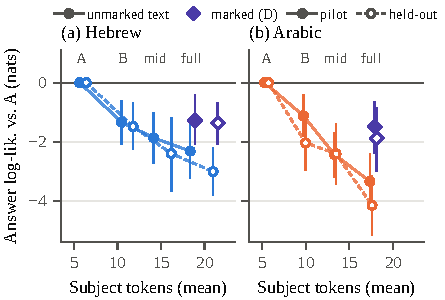
\includegraphics[width=\columnwidth]{figures/segmentation.pdf}
\caption{E6/E7, template~1, pilot and held-out cohorts by language: answer log-likelihood
relative to \cA{} for re-segmentations of the same text (\cB, \textsf{mid},
\textsf{full}: mean of the early and late splits with \cD's token count) and for
the marked prompt \cD; 95\% answer-cluster intervals.}
\label{fig:seg}
\end{figure}

\begin{table}[t]
\centering\small
\setlength{\tabcolsep}{3.2pt}
\newcommand{\estb}[3]{\makecell[c]{$#1$\\[-1pt]{\footnotesize[$#2$, $#3$]}}}
\begin{tabular}{@{}lccc@{}}
\toprule
 & \makecell{\cA$\to$\cB\\[-1pt]\footnotesize segmentation} & \makecell{\cB$\to$\cC\\[-1pt]\footnotesize positions} & \makecell{\cC$\to$\cD\\[-1pt]\footnotesize marks}\\
\midrule
\makecell[l]{Pilot\\[-1pt]Hebrew} & \estb{-1.34}{-2.11}{-0.60} & \estb{-1.12}{-1.79}{-0.44} & \estb{+1.18}{0.52}{1.87}\\[3pt]
\makecell[l]{Pilot\\[-1pt]Arabic} & \estb{-1.12}{-1.82}{-0.42} & \estb{-1.61}{-2.59}{-0.65} & \estb{+1.24}{0.36}{2.17}\\[3pt]
\makecell[l]{Held-out\\[-1pt]Hebrew} & \estb{-1.49}{-2.27}{-0.66} & \estb{-2.21}{-3.41}{-1.10} & \estb{+2.33}{1.27}{3.45}\\[3pt]
\makecell[l]{Held-out\\[-1pt]Arabic} & \estb{-2.04}{-2.99}{-1.14} & \estb{-1.42}{-2.40}{-0.45} & \estb{+1.57}{0.59}{2.59}\\
\bottomrule
\end{tabular}
\caption{E6 components (nats, template~1, relation-macro, 95\% answer-cluster
intervals); they sum to the E2 effect \cA$\to$\cD{} ($-1.28$, $-1.49$, $-1.37$,
$-1.88$).}
\label{tab:e6}
\end{table}

\textbf{Splitting further (E7).} Holding the text fixed, the group-mean
likelihood decreases across the tested levels of splitting, although some steps
between adjacent levels have intervals spanning zero (Figure~\ref{fig:seg}). At
the marked prompt's token count, the mean score of the early and late unmarked
splits, which cut letters into bytes, is 1.04 to 2.27 nats below the marked
prompt in all four pilot and held-out cohort--language groups, and every interval
excludes zero. Total token count alone therefore does not predict the likelihood across
these constructed inputs. Within this synthetic decomposition we detect no net
cost of the 7.6 to 9.2 mark tokens that marking adds on average beyond the letter
splitting they cause, whereas the same number of further, artificial splits
costs 1.0 to 2.2 nats. These exploratory analyses show sensitivity to how the
letters are split without separating count from identity: the re-splitting steps
change which tokens appear and usually how many, whereas \cB$\to$\cC{} only moves
fixed tokens. The Google-RE estimates have intervals spanning zero
(Appendix~\ref{app:extra}).

\textbf{Other tests.} Splitting a single subject token without changing the text
(E3) has a small estimated cost of a few tenths of a nat, although the intervals
permit larger ones; the pilot showed no dose-response in the number of added
tokens; and entity pairs matched on 2023 pageviews gave effects of inconsistent
sign (Appendices~\ref{app:e3} and~\ref{app:extra}).

\subsection{Where is the deficit? (RQ3)}

\begin{figure*}[t]
\centering
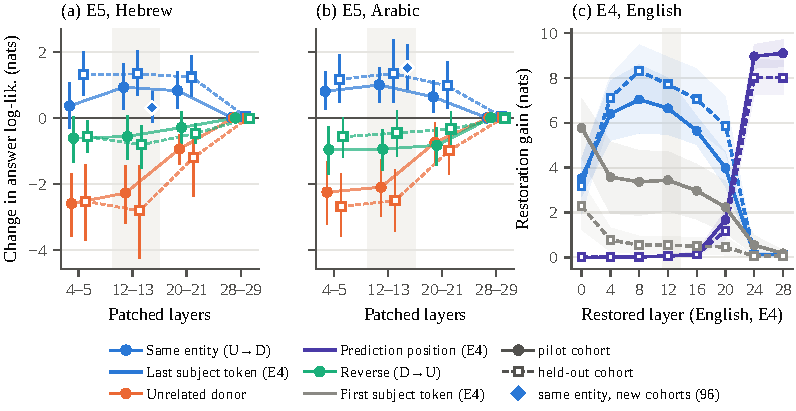
\includegraphics[width=0.8\textwidth]{figures/mechanism.pdf}
\caption{Where the deficit lives. \textbf{(a, b)} E5, template~1: change in the
gold answer's log-likelihood over the unpatched recipient (\D, or \U{} for the
reverse patch) after patching the last subject token at two layers; pilot (filled,
57 subjects), held-out (open, 40), source-checked (diamonds, 96 each). \textbf{(c)} E4 in English: gain when the clean state is restored at one
position and layer (17 pilot, 16 held-out subjects). Bars, bands: 95\% intervals.}
\label{fig:mech}
\end{figure*}

\textbf{Pilot and held-out test.} In the pilot, the declared window (layers
4--5) gave same-entity gains of 0.37 \ci{-0.31}{1.07} nats in Hebrew and 0.81
\ci{0.25}{1.39} in Arabic, and layers 12--13 gave clearer gains (0.93 and 1.00;
Figure~\ref{fig:mech}a,b). At the held-out window, fixed in advance at 12--13,
copying the unmarked state at the subject's last token into the marked run raises the log-likelihood by 1.33 \ci{0.69}{2.04} nats in Hebrew and 1.34 \ci{0.46}{2.37}
in Arabic (Holm $p=.0002$ and $.0056$). This is most of the template-1 marking
loss (1.37 and 1.88), and correct generations rise from 6 to 13 of 40 in Hebrew
and from 2 to 5 in Arabic (unmarked: 11 and 5). In the controls, the identity
sham changes the likelihood by less than 0.002 nats on average,
patches at the first subject token or the delimiter by at most 0.06, the reverse
patch lowers it ($-0.81$, $-0.45$) and the unrelated donor is strongly harmful
($-2.81$, $-2.50$). Restoration also appears at layers 4--5 and 20--21, but not at 28--29.

\textbf{Source-checked cohorts.} With the position and window unchanged, the
same-entity patch raises the Arabic margin by 1.33 \ci{0.64}{2.06} nats (Holm
$p=.0004$; Table~\ref{tab:new}), matching the marking loss of $-1.30$ nats in the
same 96 subjects. The unrelated donor lowers the margin, and the identity sham
moves it by 0.002 nats on average. In Hebrew, the same-entity and unrelated patches give similar, uncertain gains (0.36 and 0.29), so the subdistrict
task shows no entity-specific restoration.

\textbf{English localization (E4).} On the English-recallable cores, restoring the state at the subject's last token recovers 4.0 to 8.3 nats from layers 4 to 20
and almost nothing from layer 24 on, where
the prediction position takes over (Figure~\ref{fig:mech}c). This pattern of enrichment followed by extraction \citep{meng-etal-2022-locating,geva-etal-2023-dissecting} matches the layers where E5 restores marked prompts; E4 ran after E5, so
it supports the window but did not select it.

\subsection{Measurement validity}
\label{sec:validity}
The first author checked the facts and the Hebrew and Arabic spellings, and
verified the AI-assisted draft judgments against Aya's outputs and the gold
entities. In two stratified audits of 80 outputs each, the entity-correctness
judgments agreed with the automatic scorer on 79 of 80 pilot outputs, and the
held-out audit accepted 34 outputs against 19 strict matches (answer labels,
valid variants). These counts describe the samples, not full-cohort accuracy. In the Arabic cities, removing the label raises accuracy only to 28.8\% (\U) and 16.8\% (\D).

\section{Discussion}
\label{sec:discussion}

\paragraph{What replicates.} On subjects never used to develop the analysis and
on independently sourced Arabic names, marking lowers the evidence for the
correct answer by about 1.4 to 1.7 nats, and restoring the unmarked subject
state at a window chosen on the pilot recovers a comparable amount. Accuracy
moves in the same direction: the drop is significant in the exploratory pilot
test in Hebrew, large but not formally tested in the new Arabic data (23 against
4 facts answered correctly in only one form), and uncertain elsewhere. Where
measured recall
under our prompts and scoring rules is low (Google-RE, Hebrew subdistricts), the
results are inconclusive and do not establish an absence of an effect; low
baseline recall, strict matching and answer formatting are possible reasons. In
practice, entity queries should also try unmarked forms, and recall benchmarks
should include spelling variants and language-aware answer normalization.

\paragraph{What drives the loss.} E6 and E7 argue against the simplest
fragmentation account, in which each extra token dilutes the subject: within the
synthetic decomposition we detect no net cost of the mark tokens, and at equal
token count the marked name scores above artificial re-splits. The loss is
instead sensitive to how the letters are split. In \D{} the letters arrive
as short pieces, mostly single letters (10.7 pieces instead of 5.9 in pilot
Hebrew); the same pieces without marks (\cB) give an estimated loss close to
marking's, and cutting further, into bytes, costs more. This is consistent with
detokenization accounts \citep{kaplan-etal-2025-tokens,feucht-etal-2024-token},
in which the state at the subject's last token, on which enrichment builds
\citep{geva-etal-2023-dissecting}, is assembled from the pieces, so an unfamiliar
split of a familiar name may yield a less informative state, which E5 largely
restores. Weaker enrichment is one explanation consistent with our results, but
replacing the whole residual state does not separate enrichment from other
information the state carries. If this explanation holds, the written form
matters for the enrichment that \citet{fierro-etal-2025-multilingual} find to be
language-independent. Whether the opposing effects of moving tokens and
inserting marks cancel exactly remains open. Our Arabic results agree with
\citet{inoue-etal-2026-diacritics} and extend them to entity-level recall, to
Hebrew and to internal states.

\section{Limitations}
\label{sec:limits}
We study one model, in NF4 quantization, whose pretraining data are not
available, so we cannot measure directly how familiar each spelling is to it.
The reviewed cohorts have 57, 40 and 26 subjects; the pilot and held-out cohorts
both come from mLAMA, and 17 of the 40 held-out facts share an answer entity with
the pilot; final review decisions were made by one author. The source-checked cohorts cover one relation per language with a
question-first prompt, and baseline accuracy on the Hebrew relation is very low. Some
Hebrew source names are only partly marked, so that cohort tests the marking the
sources attest. Source records can be newer than Aya's training
data, so agreement between sources does not show that Aya saw a record in
training. No input manipulation
separates token count from token identity: the E6 splitting step changes both,
and forced splits and position gaps are unlike ordinary tokenizer output. The E5 window was fixed after the held-out behavioral results were
known, and whole-state patching does not separate MLP from attention.

\section{Conclusion}
Adding optional diacritics to an entity's name makes Aya-23-8B's correct answer
several times less likely, on held-out subjects and on independently sourced
Arabic city names; on Hebrew localities, where
baseline accuracy is very low, the result is inconclusive. On these held-out and
Arabic subjects, restoring the unmarked state at the subject's last token in
middle layers recovers most of the loss. Exploratory decompositions show that the loss is sensitive to how the letters are split, which a fixed cost per token does not explain, without separating count from identity.

\section*{AI Disclosure and Reflection}
\textbf{OpenAI Codex} (GPT-6, per our project
log) helped us locate potential datasets and sources, search for literature and
evidence for facts, and implement, test and debug the code. \textbf{Claude} (Anthropic, Claude
Opus 5.5) helped us draft and edit the text, correct writing mistakes, review the
writing, recheck numbers against the records, prepare figures and find issues in
our work. The
research questions, design, experiments, review decisions and interpretation are
ours; we verified all data, outputs and reported numbers and take full
responsibility for the paper.
\textbf{Contributions (Group 17).} Reviewer A led the project: she designed the
study, ran all Aya experiments on the TAU cluster, verified the data, spellings
and outputs, analyzed the results and led the writing. Reviewer B reviewed the
Arabic side of the pilot: marked spellings with sources for its 70 names, Arabic
answer names, 22 templates and source checks for 40 pilot facts. Reviewer C
verified sources for the 26 birth- and death-place pilot facts, corrected
Hebrew answer names, commented on the Hebrew and English templates and summarized
related papers.
\textbf{Reflection.} The assistants made this scale feasible and helped find
issues such as Arabic answer labels, but also proposed unsupported spellings, sources
and claims; we checked each suggestion ourselves.

\bibliography{references}

\appendix

\begin{table*}[t]
\centering\footnotesize
\setlength{\tabcolsep}{6pt}
\renewcommand{\arraystretch}{1.15}
\begin{tabular}{@{}llll@{}}
\toprule
Fact (gold answer) & & Unmarked subject (tokens) $\rightarrow$ output & Marked subject (tokens) $\rightarrow$ output\\
\midrule
McGill University (Montreal) & he & \makecell[l]{\he{אוניברסיטת מקגיל} (4)\\[-1pt]$\rightarrow$ \he{מונטריאול} \cmark} & \makecell[l]{\he{אוּנִיבֶרְסִיטַת מֶקְגִיל} (20)\\[-1pt]$\rightarrow$ \he{אירלנד} `Ireland' \xmark}\\
 & ar & \makecell[l]{\ar{جامعة مكغيل} (3)\\[-1pt]$\rightarrow$ \ar{مونتريال} \cmark} & \makecell[l]{\ar{جَامِعَة مَكْغِيل} (14)\\[-1pt]$\rightarrow$ \ar{مونتيري، كاليفورنيا.} `Monterey, CA' \xmark}\\\addlinespace[2pt]
Hapoel Haifa F.C. (Haifa) & he & \makecell[l]{\he{הפועל חיפה} (2)\\[-1pt]$\rightarrow$ \he{חיפה} \cmark} & \makecell[l]{\he{הַפּוֹעֵל חֵיפָה} (14)\\[-1pt]$\rightarrow$ \he{תל אביב-יפו} `Tel Aviv-Yafo' \xmark}\\
 & ar & \makecell[l]{\ar{هبوعيل حيفا} (6)\\[-1pt]$\rightarrow$ \ar{حيفا} \cmark} & \makecell[l]{\ar{هَبُوعِيل حَيْفَا} (14)\\[-1pt]$\rightarrow$ \ar{حيفا} \cmark}\\\addlinespace[2pt]
Alexander Cochrane (Scotland) & he & \makecell[l]{\he{אלכסנדר קוקרן} (4)\\[-1pt]$\rightarrow$ \he{אוסטרליה} `Australia' \xmark} & \makecell[l]{\he{אֲלֶכְּסַנְדֶּר קוֹקְרֶן} (22)\\[-1pt]$\rightarrow$ \he{סקוטלנד} \cmark}\\\addlinespace[2pt]
Angoul\^eme (France) & ar & \makecell[l]{\ar{أنغوليم} (3)\\[-1pt]$\rightarrow$ \ar{فرنسا} \cmark} & \makecell[l]{\ar{أَنْغُولِيم} (9)\\[-1pt]$\rightarrow$ \ar{البرتغال.} `Portugal' \xmark}\\
Kazanlak (Bulgaria) & ar & \makecell[l]{\ar{كازنلاك} (4)\\[-1pt]$\rightarrow$ \ar{بلغاريا} \cmark} & \makecell[l]{\ar{كَازَنْلَاك} (9)\\[-1pt]$\rightarrow$ \ar{أرمينيا} `Armenia' \xmark}\\
Bnei Brak (Tel Aviv subdistrict) & he & \makecell[l]{\he{בני ברק} (2)\\[-1pt]$\rightarrow$ \he{תל אביב} \cmark} & \makecell[l]{\he{בְּנֵי בְּרַק} (10)\\[-1pt]$\rightarrow$ \he{שפלת יפו-מצפון} (not a subdistrict) \xmark}\\
\bottomrule
\end{tabular}
\caption{Template-1 generations for selected pairs: pilot (first three facts) and
source-checked cohorts (last three), chosen to show harm in both languages,
Arabic robustness and one improvement. Token counts are subject-overlapping Aya
tokens; glosses are ours.}
\label{tab:examples}
\end{table*}

\section{Relation to the Proposal}
\label{app:scope}
The proposal asked whether subword fragmentation of a Hebrew or Arabic subject
weakens factual recall in Aya-23-8B, using facts from mLAMA and Wikidata, with
three broad approaches: diacritization minimal pairs, frequency-matched high-
versus low-fragmentation entities, and activation patching of the representation at the subject's last token
within a minimal pair, preceded by an English localization of
subject enrichment in the style of \citet{geva-etal-2023-dissecting}. The study
implemented these three approaches, while some of the originally proposed
mechanistic analyses remained outside the completed evaluation. A validated
enrichment score and its regression on fragmentation within frequency strata were
not completed, and confident-hallucination rates, confidence calibration and
entity-recognition steering \citep{ferrando-etal-2025-know} were not evaluated.
The English localization (E4) became a retrospective activation-restoration sweep
on the English-recallable cores of the pilot and held-out cohorts, run after E5
once a dedicated English development cohort failed its prespecified screen (4 of
14 facts recalled on both screening prompts, fewer than the required 10); it
therefore did not select the patching window through the intended
development-first procedure, and the window was chosen on the pilot instead.
Frequency matching was conducted with 2023 pageviews, but its evidence is limited
by small, relation-incomplete matched samples and by retrospective construction
for the pilot and held-out cohorts. Later implementation decisions fixed the
relations (P19, P20, P159 and P740), added a subject-disjoint held-out test frozen
before Aya was run on it and a second benchmark archive, and made the full cohorts
primary, with the proposal's English-recalled subsets retained as sensitivity
analyses rather than the inclusion criterion. The pilot was declared exploratory,
with its full-cohort contrasts as the prespecified primary analyses. The
source-checked cohorts and the E6 and E7 decompositions extend the proposal.

\section{Cohort Construction}
\label{app:cohorts}
\textbf{Marks and spelling terms.} Hebrew and Arabic are written in abjads:
letters stand for consonants, and a few letters (Hebrew \he{ו}, \he{י}; Arabic
\ar{ا}, \ar{و}, \ar{ي}) can also stand for vowels (in Arabic, long vowels). The
optional marks allowed in \D{} are, for Hebrew, the vowel points, the
\emph{dagesh} (a dot inside a letter that marks a doubled or hard consonant), the
dots that tell shin from sin (\he{שׁ}, \he{שׂ}) and the \emph{rafe} (a line that
marks a soft consonant), together called \emph{niqqud}; and, for Arabic, the short-vowel marks (\emph{fatha},
\emph{damma}, \emph{kasra}), \emph{tanwin} (doubled vowel marks for a final
\emph{-n}), \emph{shadda} (marks a doubled consonant), \emph{sukun} (no vowel) and the
\emph{dagger alif} (a small alif for a long \emph{a}). Adding these marks is
called vocalization, or \emph{pointing} for Hebrew. The marks never change the
letters: hamza (the glottal-stop sign, written alone or on a carrier letter) is
kept as written, and a Hebrew name is never switched
between full (plene) spelling, which writes some vowels with the letters \he{ו}
and \he{י}, and defective spelling, which leaves them out.

\textbf{Held-out.} Of 60 test-split candidates, 20 were rejected (by relation:
P19 4, P20 2, P159 9, P740 5): neighborhood- or state-level answers (Harlem,
Pennsylvania), a death place outside the answer city (a camp outside Beirut
municipality), organizations that moved, merged or dissolved (Cadillac, Miller,
HAPAG, the Syrian Arab Army, DuPont's headquarters outside Wilmington city
limits), subjects without a meaningful Hebrew or Arabic script form (BP, BenQ,
SNCF, SHINee, Suez, Kakao M), non-standard or truncated labels (e.g.\ an Arabic
label rendering Yona Friedman's given name as Yunus), and a person listed under
P740. Seventeen of the 40 kept facts share an answer entity with the pilot,
although no subject is shared. Item-level caveats kept in the primary analysis
are: the IRGC headquarters source gives a location only (excluded in a
sensitivity analysis, Figure~\ref{fig:forest}); San Miguel's founding place
rests on corporate continuity from an 1890 Manila brewery; the source for Tofiq
Bahramov's death place was published after Aya's release; and a few short labels
(e.g.\ Michael II, Anne Gonzaga) could denote other people.

\textbf{Google-RE.} Candidates were eligible if their subject appeared in none of
the mLAMA English, Hebrew or Arabic partitions of the four relations and their
answer entity had already been reviewed; 16 birth and 16 death candidates were
taken in a prespecified hash order from 415 and 121 eligible facts. Rejections:
two subjects whose names point to far more famous people (Tom Arnold, John Barry),
no independent source for a death place (Elisha Netanyahu), conflicting sources
(Peter Norman Nissen, Francis Alexander), and Abdülmecid I, whose only stored
answer label (Constantinople) would count the equally correct ``Istanbul'' as
wrong. Three name labels were corrected before the freeze.

\textbf{Review records.} For every candidate of the reviewed cohorts the record
holds a source URL with a pinpoint quotation, identity and answer-level checks,
and, for kept facts, both marked forms, validated mechanically against the
unmarked base letters. A 20-candidate English development sheet (14 kept) was
used only for the failed E4 screen.

\textbf{Source-checked cohorts.} Every row stores its source links and the checks
it passed. Distractors are a neighboring country where one exists, otherwise a
country on the same continent, and for Hebrew another subdistrict, from the same
district where possible. \emph{Arabic cities:} the unmarked name equals the Wikidata Arabic
label, the English gloss equals the English Wikipedia title, the Wikidata
GeoNames identifier equals the GeoNames city, the GeoNames country equals the
Wikidata country, the English name occurs among the GeoNames names or aliases,
\D{} differs from \U{} only by combining marks, and no exact GeoNames namesake
exists in another country. Of 266 linked facts, 59 were excluded for country
granularity or disputed borders, 8 for missing or disagreeing country codes and 14
for cross-country name collisions; one of the remaining 185 failed the frozen
Unicode normalization (NFC) rule. The gold country is always in its CLDR accepted-answer set, and no accepted
string belongs to two countries. The marked names carry a median of four marks
(two to eight) and add a median of six subject tokens. \emph{Hebrew localities:}
the marked form appears in the article lead, removing its marks yields the unique
official locality name, the Wikidata locality code equals the CBS code, and the
official subdistrict is nonempty. Of 646 article openings with a marked name, 21
were excluded for
disputed classification, 28 for missing or disagreeing codes and 10 because the
name contains its answer; 240 of the remaining 587 were drawn in a fixed
pseudo-random (SHA-256) order within subdistrict. The median is four marks (two to 13) and seven added tokens;
in five of 135 multiword names one word carries no marks, so this cohort tests the
marking the sources attest rather than full marking of every word. Subject
identifiers are disjoint from each other and from the reviewed cohorts, and
current pages and GeoNames records can postdate Aya's training data.

\section{Prompt Templates}
\label{app:templates}
All reviewed-cohort prompts share one three-line frame per language: ``Subject:
\{subject\}'', ``Question: \dots'' and ``Give only the place name.'' The Hebrew
frame uses \he{נושא:} (subject), \he{שאלה:} (question) and
\he{יש להשיב רק בשם המקום.}; the Arabic frame uses \ar{الموضوع:}, \ar{السؤال:} and
\ar{أجب باسم المكان فقط.} with the same meanings. Only the question varies.
Table~\ref{tab:templates} lists template~1; templates 2 and 3 paraphrase it (e.g.\
``What is this person's birthplace?''). English screening prompts use a different
form, e.g.\ ``State the birthplace of \{subject\}. Answer with only the place
name.'' The source-checked cohorts use the single-line questions of
Table~\ref{tab:templates-new}.

\begin{table*}[!ht]
\centering\small
\setlength{\tabcolsep}{6pt}
\begin{tabular}{@{}lll@{}}
\toprule
 & Arabic cities & Hebrew localities\\
\midrule
t1 & \ar{في أي دولة تقع \mbox{\{subject\}}؟ أجب باسم الدولة فقط.} & \he{באיזו נפה נמצא היישוב \mbox{\{subject\}}? השב בשם הנפה בלבד.}\\
t2 & \ar{ما الدولة التي تقع فيها \mbox{\{subject\}}؟ اكتب اسم الدولة فقط.} & \he{מה שם הנפה שבה נמצא \mbox{\{subject\}}? כתוב רק את שם הנפה.}\\
\bottomrule
\end{tabular}
\caption{Templates of the source-checked cohorts. Template~1 asks ``In which
country is \{subject\} located? Answer with the country name only.'' and ``In
which subdistrict is the locality \{subject\}? Answer with the subdistrict name
only.''; template~2 paraphrases it. English control for the Arabic cities: ``Which
country is \{subject\} located in? Give only the country's name.''}
\label{tab:templates-new}
\end{table*}

\begin{table}[!ht]
\centering\small
\setlength{\tabcolsep}{4pt}
\renewcommand{\arraystretch}{1.15}
\begin{tabular}{@{}lll@{}}
\toprule
Rel. & & Question line (template 1)\\
\midrule
\multirow{3}{*}{P19} & en & Where was this person born?\\
 & he & \he{היכן נולד האדם הזה?}\\
 & ar & \ar{أين وُلد هذا الشخص؟}\\
\midrule
\multirow{3}{*}{P20} & en & Where did this person die?\\
 & he & \he{היכן נפטר האדם הזה?}\\
 & ar & \ar{أين توفي هذا الشخص؟}\\
\midrule
\multirow{3}{*}{P159} & en & Where is this organization's headquarters?\\
 & he & \he{היכן נמצא המטה של הארגון הזה?}\\
 & ar & \ar{أين يقع المقر الرئيسي لهذه المنظمة؟}\\
\midrule
\multirow{3}{*}{P740} & en & Where was this organization founded?\\
 & he & \he{היכן נוסד הארגון הזה?}\\
 & ar & \ar{أين تأسست هذه المنظمة؟}\\
\bottomrule
\end{tabular}
\caption{Question line of evaluation template~1 per relation and language in the
reviewed cohorts.}
\label{tab:templates}
\end{table}

\section{Same-Text Resegmentation (E3)}
\label{app:e3}
E3 replaces one token of an unmarked template-1 prompt by two vocabulary tokens
that decode to exactly the same bytes, either inside the subject (In) or outside
it (Out), which holds the added length constant. In the pilot a matched control
existed only in Arabic, where In$-$Out was $-0.61$ nats. On the held-out subjects
In$-$Out is $-0.43$ nats with the original rule and $-0.53$ with a byte-level rule
that also yields Hebrew controls ($-0.18$, interval spanning zero; Holm $p=.067$
and $.288$). Relative to the canonical tokenization, the subject split costs
little ($-0.07$ to $-0.25$ nats), whereas outside splits \emph{raise} the Arabic
answer's likelihood ($+0.36$), mostly for place-of-death facts; moving the
outside split to the nearest feasible token before or after the subject gives
similar contrasts ($-0.62$ and $-0.74$), again driven by the control arm. The
estimated cost of a single non-canonical boundary inside a name is small, although
the confidence intervals permit larger decreases; in E6 and E7 the estimated cost
grows as the letters are cut more finely.

\begin{table}[!ht]
\centering\footnotesize
\setlength{\tabcolsep}{2.2pt}
\begin{tabular}{@{}lccc@{}}
\toprule
Cohort (lang) & In$-$Out & In$-$Can & Out$-$Can\\
\midrule
Pilot (ar) & \est{-0.61}{-1.03}{-0.24} & \est{-0.39}{-0.80}{-0.02} & \est{0.23}{0.04}{0.40}\\
Held-out (ar) & \est{-0.43}{-0.86}{0.04} & \est{-0.07}{-0.50}{0.41} & \est{0.36}{0.15}{0.57}\\
Held-out$^b$ (he) & \est{-0.18}{-0.50}{0.15} & \est{-0.25}{-0.60}{0.11} & \est{-0.06}{-0.16}{0.03}\\
Held-out$^b$ (ar) & \est{-0.53}{-0.98}{-0.03} & \est{-0.17}{-0.63}{0.33} & \est{0.36}{0.15}{0.57}\\
\bottomrule
\end{tabular}
\caption{E3: change in canonical-answer log-likelihood (nats) when one token is
split inside the subject (In) or outside it (Out), relative to each other or to
the canonical tokenization (Can). $^b$Byte-level rule; the original rule found
no valid Hebrew outside split (Hebrew In$-$Can $-0.26$ \ci{-0.70}{0.21}, 30
subjects).}
\label{tab:e3}
\end{table}

\section{Additional Results}
\label{app:extra}

\paragraph{Robustness of E2.} Figure~\ref{fig:forest} collects the E2 sensitivity
analyses of the reviewed cohorts. The held-out likelihood loss lies between
$-1.37$ and $-1.46$ nats (Hebrew) and $-1.38$ and $-1.88$ nats (Arabic) under each
template, keeps its size on the English-recallable core ($-1.30$ and $-1.31$; the
Arabic interval with 16 subjects includes zero), and survives excluding a
headquarters fact with a location-only source and a subject whose name contains
its answer. With the answer-label rule, fixed after the pilot and before the
held-out outputs, the held-out Arabic accuracy effect is $-11.5$ points
\ci{-25.6}{2.6}.

\begin{figure*}[!ht]
\centering
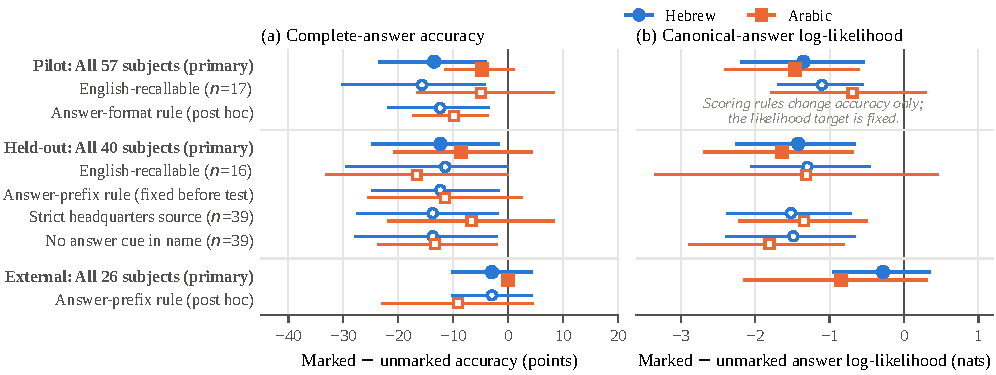
\includegraphics[width=0.92\textwidth]{figures/forest_effects.pdf}
\caption{Robustness of the marked-minus-unmarked effect (E2) in the reviewed
cohorts. Points are relation-macro estimates with 95\% subject-cluster bootstrap
intervals; filled markers are the prespecified primary analyses, hollow markers
sensitivity analyses. English-recallable cores are selected by two separate
English screening prompts. Answer-format rules strip one Arabic answer label
(and, in the pilot, one Hebrew sentence frame) before exact matching.}
\label{fig:forest}
\end{figure*}

\paragraph{Margins in the reviewed cohorts.} The post hoc margin over one
same-relation distractor per fact falls by $-1.82$ \ci{-2.90}{-0.68} and $-2.11$
\ci{-3.41}{-0.94} nats in the pilot, $-3.01$ \ci{-4.32}{-1.77} and $-2.48$
\ci{-3.88}{-1.22} on the held-out subjects and $-0.98$ \ci{-1.99}{0.08} and
$-1.11$ \ci{-2.80}{0.45} on Google-RE (Hebrew, Arabic), while the distractor's own
log-likelihood rises by 0.26 to 1.59 nats.

\paragraph{Source-checked cohorts.} Subject-weighted means give the same signs as
the stratum-macro estimates in Table~\ref{tab:new} ($\Delta M$ $-0.99$ Arabic,
$-0.19$ Hebrew). In the Arabic cities the distractor's log-likelihood also falls,
by 0.37 nats, so the margin loss reflects a larger fall of the gold answer
($-1.74$). With the answer-label rule, 53 and 31 of 184 Arabic answers (\U,
\D) are correct; for Hebrew, 9 and 4 of 240. The E5 first-subject patch changes
the margin by $-0.03$ (Arabic) and $0.00$ (Hebrew) nats, and the same-entity gain
in the gold answer's own log-likelihood is 1.52 \ci{0.86}{2.22} and 0.31
\ci{-0.15}{0.82} nats (the diamonds in Figure~\ref{fig:mech}).

\paragraph{E6 and E7 by cohort and language.} The same-count contrast \cD$-$\textsf{full} is
$+1.04$ \ci{0.45}{1.65} and $+1.85$ \ci{1.04}{2.70} in the pilot (Hebrew, Arabic)
and $+1.65$ \ci{0.75}{2.60} and $+2.27$ \ci{1.28}{3.24} on the held-out subjects;
early minus late lies between $+0.09$ and $+0.78$, every interval spanning zero.
In Arabic, 53 to 64\% of the subject tokens of the \textsf{full} splits are
partial UTF-8 characters, against none in \D.
In the 26-subject Google-RE cohort every E6 component and \cD$-$\textsf{full}
interval spans zero. Hebrew: \cA$\to$\cB{} $-0.49$, \cB$\to$\cC{} $-0.49$,
\cC$\to$\cD{} $+0.54$, \cD$-$\textsf{full} $+0.35$ nats; Arabic: $-0.63$, $+0.17$,
$-0.39$ and $+0.43$. In all six cohort--language groups, the \textsf{mid} and \textsf{full}
splits have exactly the planned subject-token counts, and \cA{} and \cB{} have the
same subject-token count for only 4 of 246 pairs.

\paragraph{Errors.} Aya did not abstain in any condition; its errors are
plausible-looking place substitutions (Table~\ref{tab:examples}). Across all wrong
pilot E2 answers the most frequent outputs are New York in Hebrew (25 of 301) and
Berlin in Arabic (22 of 306), and Arabic errors include country names. In 11 of
171 pilot Hebrew \D{} generations (none with \U) the model copied niqqud into its
answer.

\paragraph{Relation-level and frequency results.}
Table~\ref{tab:relations} breaks the pilot and held-out E2 likelihood effects
down by relation, Table~\ref{tab:freq} gives the pilot frequency-only baseline,
Table~\ref{tab:e5} lists the E5 estimates of both reviewed cohorts, and
Figure~\ref{fig:tok} shows the token counts per subject. In E4, restoring the
state at the subject's last token in layer 12 recovers 6.64 nats on the pilot core and 7.71 on
the held-out core.

\begin{table}[!ht]
\centering\small
\setlength{\tabcolsep}{2.4pt}
\begin{tabular}{llcc}
\toprule
 & Rel. & Pilot $\Delta S$ & Held-out $\Delta S$\\
\midrule
he & P19  & $-0.68$ \ci{-2.76}{1.46} & $-0.84$ \ci{-2.14}{0.34}\\
he & P20  & $-0.48$ \ci{-1.92}{1.01} & $-1.43$ \ci{-2.39}{-0.55}\\
he & P159 & $-3.09$ \ci{-4.72}{-1.48} & $-1.54$ \ci{-3.32}{0.08}\\
he & P740 & $-1.16$ \ci{-2.28}{0.04} & $-1.88$ \ci{-3.84}{-0.07}\\
ar & P19  & $-0.45$ \ci{-1.99}{1.15} & $-0.58$ \ci{-1.90}{0.73}\\
ar & P20  & $-0.95$ \ci{-2.28}{0.27} & $-1.18$ \ci{-3.04}{0.70}\\
ar & P159 & $-1.81$ \ci{-4.38}{0.13} & $-2.63$ \ci{-5.37}{-0.21}\\
ar & P740 & $-2.66$ \ci{-4.29}{-1.06} & $-2.16$ \ci{-3.80}{-0.95}\\
\bottomrule
\end{tabular}
\caption{E2 likelihood effects (nats) by relation (descriptive; pilot 14--15 and
held-out 6--13 subjects per relation). Organization names (P159) receive the
most added tokens.}
\label{tab:relations}
\end{table}

\begin{table}[!ht]
\centering\small
\setlength{\tabcolsep}{4pt}
\begin{tabular}{lccc}
\toprule
Predictor & English & Hebrew & Arabic\\
\midrule
log sitelinks & \est{0.65}{0.49}{0.80} & \est{0.56}{0.39}{0.72} & \est{0.45}{0.30}{0.60}\\
fewer \U{} tokens & \est{0.43}{0.29}{0.59} & \est{0.31}{0.14}{0.51} & \est{0.46}{0.27}{0.64}\\
\midrule
recalled subjects & 34/57 & 12/57 & 9/57\\
\bottomrule
\end{tabular}
\caption{Post-hoc frequency-only baseline on the pilot: AUROC of single
subject-level predictors for recalling a fact with the unmarked name in at least
one of three templates (95\% subject bootstrap intervals).}
\label{tab:freq}
\end{table}

\begin{table}[!ht]
\centering\scriptsize
\setlength{\tabcolsep}{2.1pt}
\begin{tabular}{@{}lrrrr@{}}
\toprule
Condition & 4--5 & 12--13 & 20--21 & 28--29\\
\midrule
\multicolumn{5}{l}{\emph{Hebrew, pilot / held-out}}\\
Same entity & 0.37/1.31 & 0.93/1.33 & 0.83/1.24 & 0.01/0.03\\
Unrelated & $-$2.59/$-$2.52 & $-$2.27/$-$2.81 & $-$0.94/$-$1.20 & 0.00/$-$0.01\\
Reverse & $-$0.61/$-$0.57 & $-$0.56/$-$0.81 & $-$0.29/$-$0.46 & 0.00/$-$0.01\\
First subj. & $-$0.01/0.03 & $-$0.02/0.03 & $-$0.05/0.01 & $-$0.01/$-$0.01\\
Delimiter & 0.10/0.01 & 0.08/0.06 & 0.05/0.08 & 0.01/0.03\\
\midrule
\multicolumn{5}{l}{\emph{Arabic, pilot / held-out}}\\
Same entity & 0.81/1.17 & 1.00/1.34 & 0.64/0.97 & 0.00/0.05\\
Unrelated & $-$2.24/$-$2.68 & $-$2.09/$-$2.50 & $-$0.74/$-$1.00 & 0.01/0.01\\
Reverse & $-$0.96/$-$0.57 & $-$0.94/$-$0.45 & $-$0.83/$-$0.33 & 0.00/0.00\\
First subj. & $-$0.01/0.13 & 0.03/0.00 & 0.04/$-$0.01 & 0.00/0.01\\
Delimiter & $-$0.15/0.01 & 0.01/0.05 & $-$0.01/0.02 & 0.00/0.00\\
\bottomrule
\end{tabular}
\caption{E5 mean change in canonical-answer log-likelihood (nats) by window,
pilot / held-out. Identity shams are within $\pm0.002$ everywhere. Unpatched
template-1 baselines (correct of $n$): pilot Hebrew 2 (\D) and 12 (\U), Arabic 5
and 8 of 57; held-out Hebrew 6 and 11, Arabic 2 and 5 of 40.}
\label{tab:e5}
\end{table}

\begin{figure}[!ht]
\centering
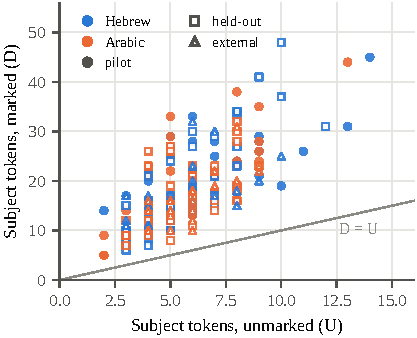
\includegraphics[width=\columnwidth]{figures/tokenization.pdf}
\caption{Subject-overlapping Aya tokens per subject (mean of three templates),
unmarked versus marked, in the reviewed cohorts. Every point lies above the
diagonal.}
\label{fig:tok}
\end{figure}

\paragraph{Frequency matching.} Pairs were formed within relation and language
between subjects above and below the pilot's median unmarked token density,
matching log 2023 pageviews (caliper 1.5) and base-letter length (caliper 5).
Pilot and held-out pairs were formed after outcomes existed but without using
them; Google-RE pairs were frozen before any Google-RE output. High-minus-low unmarked
accuracy: pilot $+1.7$ (he, 20 pairs) and $-5.1$ points (ar, 13); held-out
$-23.8$ \ci{-42.9}{-4.8} (he, 14) and $-6.7$ \ci{-20.0}{0.0} (ar, 10); Google-RE
$+16.7$ \ci{-8.3}{45.8} (he, 8) and 0.0 (ar, 7; no strict matches). High-minus-low
answer likelihood: held-out $-1.17$ and $-0.96$ nats; Google-RE $+2.36$
\ci{0.64}{4.05} and $-1.62$ \ci{-3.33}{-0.11}. Intervals resample pairs within
relation and omit matching uncertainty.

\end{document}
